\documentclass[11pt,paper=letter]{scrartcl}
\usepackage[wide,noextlink]{cjquines}
\usepackage{tkz-graph}
% tkz-graph is no longer in distribution, but the latest stable version will still compile this file

\newcommand{\crs}[1]{\mathrm{cr}(#1)}

\begin{document}

\title{Crossing numbers}
\author{Carl Joshua Quines}
\date{August 22, 2016}

\maketitle

\begin{abstract}
This article discusses crossing numbers, the Euler characteristic of graphs, Kuratowski's, Wagner's and F\'{a}ry's theorems, ultimately leading up to a discussion of the crossing number inequality.
\end{abstract}

\section{A motivating puzzle}

One of the classical mathematical puzzles is the three utility problem, which can be phrased as follows:

\begin{problem}[Three utility problem]
Suppose that three houses are on a field, and each needs to be connected to gas, water and electricity companies. Without using a third dimension or sending any of the connections through a company or a house, find a way to make all nine connections without any of the lines crossing each other.
\end{problem}

\begin{center}
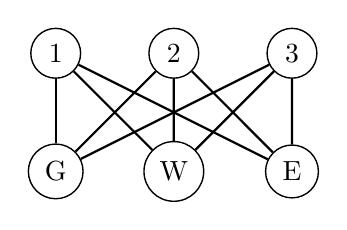
\begin{tikzpicture}[scale=1.5]
\GraphInit[vstyle=Normal]
\Vertex{1} \EA(1){2} \EA(2){3}
\SO(1){G} \EA(G){W} \EA(W){E}
\Edges(1,G,2,W,1,E,2) \Edge(3)(G) \Edge(3)(W) \Edge(3)(E)
\end{tikzpicture}
\end{center}

The reader who has not seen this problem before is advised to try it out. In other words, the problem asks for a way to draw the diagram above such that no of the lines cross each other.

The answer to this puzzle is \emph{no}. As in, there is no way to do this -- any drawing of such a connection will have at least one pair of lines crossing each other. However, the answer alone is unsatisfying. It does not illuminate as to the reason \emph{why} such a drawing is impossible.

The purpose of this article is to delve into the mathematical formulation behind the three utility problem: by representing the houses and companies as vertices and the connections as edges, we produce a graph. The article develops the tools to solve the three utility problem, and problems similar to this.

A note: a primary focus of this article is to illuminate the \emph{motivation} behind the proofs presented. The various heuristics used in the proofs is shown, as these appear regularly in other combinatorial arguments, and more generally in problem solving, particularly in competitive mathematics.

\section{Crossing numbers}

We define a \emph{graph} as a collection of \emph{vertices} and \emph{edges} connecting pairs of these vertices. For the remainder of this article, we assume the graph is \emph{undirected} (edges do not have a particular direction), \emph{connected} (by following edges, we can get from one vertex to any other vertex), \emph{loop-free} (no edge connects a vertex to itself), and \emph{multiplicity-free} (no pair of vertices is connected by more than one edge).

The simplest way to represent a graph is a plane drawing. A typical plane drawing of a graph will indicate vertices using dots, and edges as curves with dots as the endpoints. Now, there are an infinite number of ways to draw a graph, but in this article, our interest is drawn to the drawing with the least number of crossings. A \emph{crossing} in a drawing occurs when two edges overlap.

We define the crossing number $\crs{G}$ of a graph $G$ as the minimum number of crossings in a planar drawing of $G$. When we can draw a graph $G$ such that none of its edges cross, equivalently, when $\crs{G} = 0$, we say that $G$ is \emph{planar}.

Suppose we have a graph with $n$ vertices and draw an edge between every pair of distinct vertices. This graph is $K_n$, the \emph{complete graph} with $n$ vertices.

Say we have a set of $m$ vertices and a set of $n$ vertices, and draw an edge between all pairs of two vertices from different sets. This graph is $K_{m, n}$, the \emph{complete bipartite graph} with $m$ vertices in one set and $n$ vertices in the other.

The observant reader will notice that the graph described in the three utility problem above is, in fact, $K_{3, 3}$, and the problem is asking to show that $K_{3, 3}$ is planar. In fact, another name for $K_{3,3}$ is the \emph{utility graph}. We will get to the proof that $K_{3, 3}$ is not planar after a few preliminary problems. The first problem we present is a simple one, which the reader should try:

\begin{problem}
Show that $K_4$ is planar.
\end{problem}

\begin{proof}
After a few attempts of drawing $K_4$, we notice that there is a configuration with no crossings. And behold, here is our proof:

\begin{center}
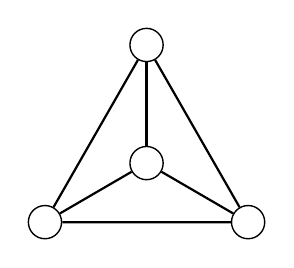
\begin{tikzpicture}[scale=1.5]
\GraphInit[vstyle=Hasse]
\Vertex{A}
\Vertex[x=0,y=1]{B} \Vertex[x=-.86,y=-.5]{C} \Vertex[x=.86,y=-.5]{D}
\Edges(A,B,C,D,A,C) \Edge(B)(D)
\end{tikzpicture}
\end{center}
\end{proof}

\begin{problem}
Show that $\crs{K_5}$ is $1$.
\end{problem}

\begin{proof}
After playing around, we can find a drawing of $K_5$ that has only one crossing:

\begin{center}
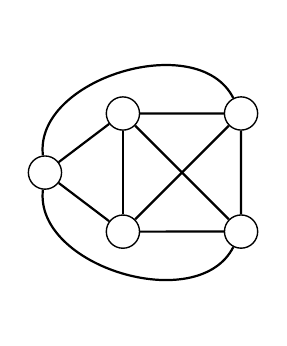
\begin{tikzpicture}[scale=1.5]
\GraphInit[vstyle=Hasse]
\Vertex{A} \NO(A){B} \EA(B){C} \SO(C){D} \Vertex[x=-.66,y=.5]{E}
\Edges(A,B,C,D,A,C) \Edge(B)(D) \Edge(E)(A) \Edge(E)(B)
\Edge[style={bend right=80}](E)(D) \Edge[style={bend left=80}](E)(C)
\end{tikzpicture}
\end{center}

This, however, is not a full proof. The diagram only proves that $\crs{K_5} \leq 1$. To complete our proof, we need to show that $\crs{K_5} \geq 1$ -- or in other words, we need to show that the crossing number of $K_5$ can't be zero, that it isn't planar.

Observe that if a drawing of $K_5$ is planar, then we can take away one vertex and all the edges connected to that vertex to get $K_4$. Since the original graph, $K_5$, is planar, then the graph formed by removing one vertex, $K_4$, must also be planar. Thus, to draw a planar graph of $K_5$, we can instead consider a planar drawing of $K_4$.

\begin{center}
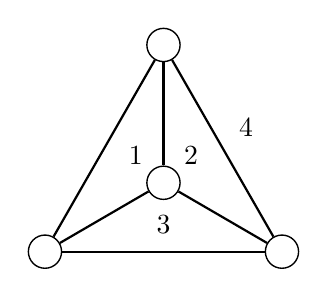
\begin{tikzpicture}[scale=1.75]
\GraphInit[vstyle=Hasse]
\Vertex{A}
\Vertex[x=0,y=1]{B} \Vertex[x=-.86,y=-.5]{C} \Vertex[x=.86,y=-.5]{D}
\Edges(A,B,C,D,A,C) \Edge(B)(D)
\draw (-.2,.2) node {1};
\draw (.2,.2) node {2};
\draw (0,-.3) node {3};
\draw (.6,.4) node {4};
\end{tikzpicture}
\end{center}

Consider the above planar drawing of $K_4$. The fifth vertex needed to make $K_5$ must end up in one of the four regions shown above, either one of the three internal regions 1, 2, or 3, or the large external region 4.

In either case, the vertex will be enclosed by a triangular region, formed by three vertices and three edges. To draw an edge from the fifth vertex to the other vertex, we have to cross one of the edges of $K_4$ -- contradicting the fact that $K_5$ is planar. Thus, we have shown that $K_5$ is not planar, so $\crs{K_5} \geq 1$. Combined with $\crs{K_5} \leq 1$, we have $\crs{K_5} = 1$.
\end{proof}

The crux idea of this proof is to make use of the fact that any part of a planar graph is still planar. This makes use of the heuristic of \emph{decomposing and recombining}. We look at the problem of proving that $K_5$ is non-planar, and we recall our previous result, that $K_4$ is planar, which turns out to be useful.

These tools -- the idea of looking at a part of a graph, and the heuristic of decomposing and recombining -- are in fact sufficient to solve the three utility problem. The reader is urged to try the problem first, before reading the solution presented below. 

\begin{problem}[Three utility problem]
Show that $\crs{K_{3,3}}$ is $1$.
\end{problem}

\begin{proof}
We observe that this problem is similar to the previous problem. This gives us the inspiration to use a similar approach: first prove the upper bound of $\crs{K_{3,3}}$ through a diagram, then prove the lower bound by using a part of $\crs{K_{3,3}}$ which is planar. After experimentation, we notice that $K_{3,2}$ is planar, which leads to the following solution.

The following diagram is $K_{3,3}$ with only one crossing, which establishes the bound of $\crs{K_{3,3}} \leq 1$. The two sets of vertices are colored gray and white.

\begin{center}
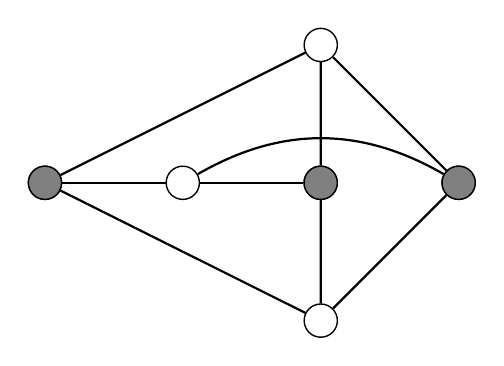
\begin{tikzpicture}[scale=1.75]
\GraphInit[vstyle=Hasse]
\Vertex{A} \EA(A){F} \EA(F){B} \EA(B){C}
\NO(B){D} \SO(B){E}
\Edges(A,D,B,E,A) \Edges(D,C,E)
\Edges(A,F,B) \Edge[style=bend left](F)(C)
\AddVertexColor{gray}{A,B,C}
\end{tikzpicture}
\end{center}

In a similar manner to the above proof of $\crs{K_5} = 1$, we start with a planar drawing of $K_{3,2}$, and add a vertex.

\begin{center}
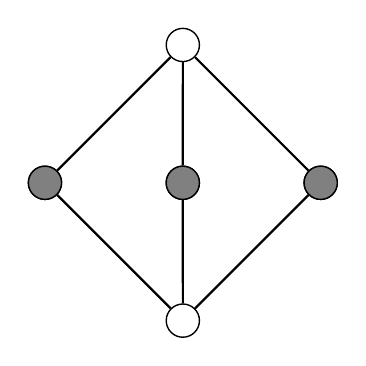
\begin{tikzpicture}[scale=1.75]
\GraphInit[vstyle=Hasse]
\Vertex{A} \EA(A){B} \EA(B){C}
\NO(B){D} \SO(B){E}
\Edges(A,D,B,E,A) \Edges(D,C,E)
\AddVertexColor{gray}{A,B,C}
\end{tikzpicture}
\end{center}

Through similar logic, wherever we place the additional vertex, we need to cross an edge. Thus the graph of $K_{3, 3}$ is not planar, and so $\crs{K_{3,3}} \geq 1$. Combined with the fact that $\crs{K_{3,3}} \leq 1$, this means that $\crs{K_{3,3}} = 1$.
\end{proof}

These two problems illustrate the heuristic of \emph{looking at sub-problems}: choosing sub-problems that are easier to solve than our original problem and using the results to solve the original. Another strategy used is \emph{trying specific cases}: drawing graphs similar to the one in the original problem, in order to look for a solution.

One of the questions, perhaps, is why we chose to look at $K_{3,2}$ rather than any other graph. Lots of graphs are planar -- why this particular graph? Well, $K_{3,2}$ is a \emph{large} part of this problem -- it is only one vertex away from $K_{3,3}$. After proving the planarity of $K_{3,2}$, we are already halfway to the problem of proving $\crs{K_{3,3}} = 1$.

When choosing sub-problems, we generally do not want to pick a sub-problem that is too small or too specific compared to the problem we want to solve, otherwise, the results we derive might prove to be unrelated, or unhelpful to the original problem. On the other hand, when the sub-problem is chosen well, the problem might already be nearly finished. Sometimes figuring out what sub-results to prove is harder than actually proving them!

At this point, the reader might be dissatisfied with the amount of rigor present in the above solutions. We will come back with a more rigorous approach to these two problems, proving that $\crs{K_5}$ and $\crs{K_{3,3}}$ are both $1$, in the next section, where we develop the Euler characteristic.

\section{The Euler characteristic}

Readers familiar with the Euler characteristic will recognize its definition in polyhedra. Indeed, it is a well-known result that in any convex polyhedron, the number of vertices minus the number of edges plus the number of faces is equal to two. In formula form, we have $V - E + F = 2$, where $V$ is the number of vertices, $E$ is the number of edges, and $F$ is the number of faces.

In this equation, the constant $V - E + F$ is known as the \emph{Euler characteristic}, and is usually denoted by $\chi$. The Euler characteristic of convex polyhedra, as above, is $2$, while non-convex polyhedra usually have a variety of Euler characteristics. Since $\chi = 2$ for any convex polyhedron, we can use Euler's characteristic to prove that there are only five Platonic solids, which is presented as further reading. \cite{fleck}

But how does this relate to graphs? Observe the two diagrams below. The left diagram is a drawing of a cube, while the right diagram is the same graph as the left after rearranging the vertices.

\begin{center}
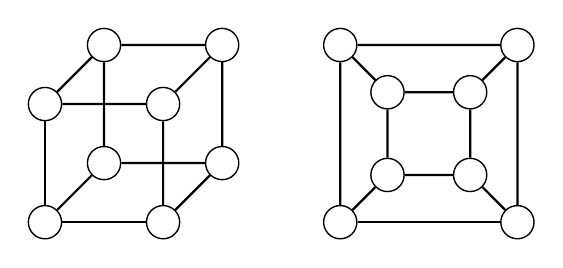
\begin{tikzpicture}[scale=1.5]
\GraphInit[vstyle=Hasse]
\Vertex{1} \NO(1){2} \Vertex[x=.5,y=1.5]{3} \EA(3){4} \EA(2){5}
\SO(3){6} \EA(6){7} \EA(1){8}
\Edges(1,2,5,8,1,6,7,4,3,6) \Edge(2)(3) \Edge(5)(4) \Edge(7)(8)
\Vertex[x=2.5,y=0]{1'} \Vertex[x=4,y=0]{8'} \Vertex[x=2.5,y=1.5]{2'}
\Vertex[x=4,y=1.5]{5'} \Vertex[x=2.9,y=.4]{6'} \Vertex[x=3.6,y=.4]{7'}
\Vertex[x=2.9,y=1.1]{3'} \Vertex[x=3.6,y=1.1]{4'}
\Edges(1',2',5',8',1',6',7',4',3',6') \Edge(2')(3') \Edge(5')(4') \Edge(7')(8')
\end{tikzpicture}
\end{center}

Notice that the graph is planar -- in other words, if we represent the vertices and edges of a cube as a graph, we produce a planar graph. The faces of the cube also have analogous ``faces'' in the graph: the regions enclosed by edges, of which both graphs have six (taking care to count the large, external region as a face).

Thus both the cube and its graph have the same Euler characteristic: $2$. Notice further that $K_4$ is a graph of the tetrahedron, so using an analogous definition for faces, $K_4$ has an Euler characteristic of $2$. A little more experimentation will show that the octahedron also has a planar graph, and so does the dodecahedron -- so these graphs have an Euler characteristic of $2$ as well.

\begin{center}
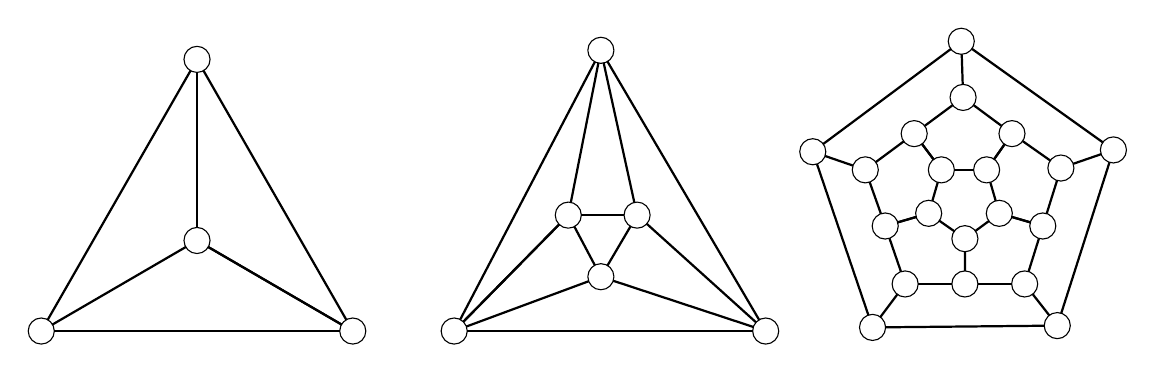
\begin{tikzpicture}[scale=2.3]
\GraphInit[vstyle=Hasse]
\tikzset{VertexStyle/.style = {shape = circle, minimum size = 3 pt, draw}}
\Vertex{1} \Vertex[x=0,y=1]{2} \Vertex[x=-0.86,y=-0.5]{3} \Vertex[x=0.86,y=-0.5]{4}
\Vertex[x=1.42,y=-0.5]{5} \Vertex[x=3.14,y=-0.5]{6} \Vertex[x=2.23,y=1.05]{7} \Vertex[x=2.05,y=0.14]{8} \Vertex[x=2.43,y=0.14]{9} \Vertex[x=2.23,y=-0.20]{10}
\Vertex[x=3.73,y=-0.48]{11} \Vertex[x=3.4,y=0.49]{12} \Vertex[x=4.22,y=1.1]{13} \Vertex[x=5.06,y=0.5]{14} \Vertex[x=4.75,y=-0.47]{15}
\Vertex[x=3.91,y=-0.24]{16} \Vertex[x=3.8,y=0.08]{17} \Vertex[x=3.69,y=0.39]{18} \Vertex[x=3.96,y=0.59]{19} \Vertex[x=4.23,y=0.79]{20}
\Vertex[x=4.5,y=0.59]{21} \Vertex[x=4.77,y=0.4]{22} \Vertex[x=4.67,y=0.08]{23} \Vertex[x=4.57,y=-0.24]{24} \Vertex[x=4.24,y=-0.24]{25}
\Vertex[x=4.04,y=0.15]{26} \Vertex[x=4.11,y=0.39]{27} \Vertex[x=4.36,y=0.39]{28} \Vertex[x=4.43,y=0.15]{29} \Vertex[x=4.24,y=0.01]{30}

\Edges(1,2,4,3,2,1,4,1,3) \Edges(5,6,7,5,8,7,9,6,10,5,8,9,10,8) \Edges(11,12,13,14,15,11) \Edge(11)(16) \Edge(12)(18) \Edge(13)(20) \Edge(14)(22) \Edge(15)(24) \Edges(16,17,18,19,20,21,22,23,24,25,16) \Edges(25,30,26,17,26,27,19,27,28,21,28,29,23,29,30)
\end{tikzpicture}
\end{center}

This gives us the inspiration to examine the Euler characteristic for planar graphs, after defining a face. We define a \emph{face} in a graph as the mutually exclusive regions enclosed by edges. Using this definition, one can be lead to the natural conjecture that, for planar graphs, $\chi = 2$. We will set out to prove this fact using induction. The reader will do well to try an inductive proof of his own before reading the proof below.

\begin{problem}
Show that the Euler characteristic for planar graphs is $2$.
\end{problem}

\begin{proof}
Some definitions first: a \emph{cycle} is a series of vertices that start and end with the same vertex, such that each consecutive pair of vertices is connected by an edge. A \emph{tree} is a graph that does not have any cycles.

\begin{center}
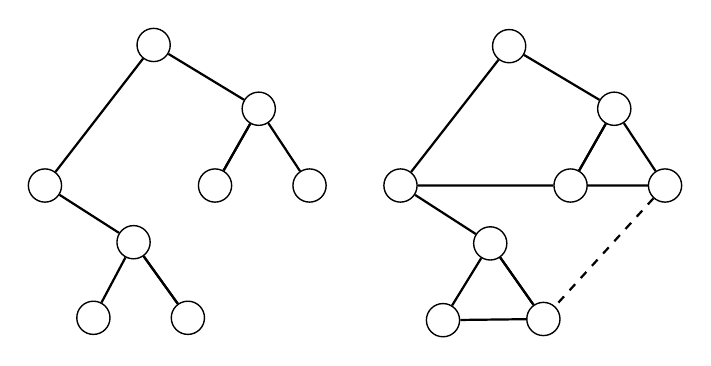
\begin{tikzpicture}[scale=1.5]
\GraphInit[vstyle=Hasse]
\Vertex[x=0.51,y=2.31]{1} \Vertex[x=1.4,y=1.77]{2} \Vertex[x=-0.41,y=1.12]{3} \Vertex[x=1.03,y=1.12]{4} \Vertex[x=1.83,y=1.12]{5} \Vertex[x=0.34,y=0.64]{6} \Vertex[x=0,y=0]{7} \Vertex[x=0.8,y=0]{8}
\Edges(7,6,8,6,3,1,2,4,2,5)

\Vertex[x=3.52,y=2.3]{11} \Vertex[x=4.41,y=1.77]{12} \Vertex[x=2.6,y=1.12]{13} \Vertex[x=4.04,y=1.12]{14} \Vertex[x=4.84,y=1.12]{15} \Vertex[x=3.36,y=0.63]{16} \Vertex[x=2.96,y=-0.02]{17} \Vertex[x=3.81,y=-0.01]{18} 
\Edges(17,16,18,16,13,11,12,14,12,15)
\Edges(13,14,15) \Edge(17)(18) \Edge[style=dashed](15)(18)
\end{tikzpicture}
\end{center}

We will proceed by induction on $F$, the number of faces. The base case, when $F = 1$, is when the graph is a tree, for which $V = E + 1$. For the induction step, suppose that $\chi = 2$ for all planar graphs with $F$ faces. Suppose we have a graph with $F+1$ faces. We choose an edge that has two distinct faces on either side, and remove that edge. This edge exists until the graph is not a tree -- if it did not exist, that meant all edges have the same face on either side, meaning the graph is a tree. This reduces the number of edges by $1$ and the number of faces by $1$, which keeps $\chi$ constant.
\end{proof}

The main idea in this proof is the use of induction. Induction is a very helpful tool, which appears often in mathematical proofs. A proof of the Euler characteristic can also be done through induction on the number of vertices, or induction on the number of edges, several of which are presented as further reading. \cite{wikipedia}

In general, when doing induction on combinatorial problems, we want to choose an object with specific properties. In this case, we chose an edge that has a distinct face on either side, and took that out, rather than just any edge. When inducting in a graph theory problem, for example, we might choose to take out the vertex with the highest or lowest degree.

We use the Euler characteristic to present a formal proof of $\crs{K_{3,3}} = 1$. The idea is to use the Euler characteristic to find bounds on $F$, then looking for a contradiction. The interested reader should try this out before reading the proof presented below.

\begin{problem}
Use the Euler characteristic to provide an alternate proof for $\crs{K_{3,3}} = 1$.
\end{problem}

\begin{proof}
Prove the upper bound as previously, by drawing a diagram. To prove the lower bound, we note that in $K_{3,3}$, each face must have at least four edges. If a face had only three edges, then there would be three edges that form a triangle, but there aren't any triangles in $K_{3,3}$.

We use the fact that $\chi = 2$: since $K_{3,3}$ has $6$ vertices and $9$ edges, a planar drawing will have $5$ faces. Each face has at least four edges, so we get at least $20$ edges -- but we've overcounted, since each edge has a face on either side. Thus the graph must have at least $10$ edges, contradicting the fact that it has $9$ edges.
\end{proof}

Again, the idea was a proof by contradiction. Here we achieve a contradiction through the technique of \emph{counting in two ways}. We count the number of edges $E$, first by looking at the graph itself, and second by using the fact that the number of faces and edges are related, the same technique that will be used in the next problem.

From this problem, we see that the number of faces and edges in a planar graph are related. Each face is enclosed by at least three edges, and each edge has at most two faces on either side. This idea is used in the problem below, for which the same technique is used, but generalized to any planar graph. The reader should keep the method used in the previous problem in mind, and try out the next problem before reading the solution presented.

\begin{problem}
For a planar graph, show that $E \leq 3V - 6$.
\end{problem}

\begin{proof}
In a planar graph, a face is enclosed by at least three edges, and an edge has at most two faces on either side. Thus you have the inequality $2E \geq 3F$ -- the number of edges would be at least thrice the number of faces, but we overcounted because an edge has at most two faces on either side. Using this and the fact that $\chi = V - E + F = 2$, it follows after some manipulation that $E \leq 3V - 6$.
\end{proof}

Once again, in this proof we used the technique of counting in two ways: counting the number of edges $E$, first by using the fact that the number of edges and faces are related, and second, finishing off with an application of the Euler characteristic.

The above inequality is quite useful, as we will see later on in the proof of the crossing number inequality. Meanwhile, we use this inequality to obtain a more rigorous proof of a previous result. The reader is advised once again to try this problem out, as it is a straightforward application of the above inequality.

\begin{problem}
Use the above inequality to provide an alternate proof for $\crs{K_5} = 1$.
\end{problem}

\begin{proof}
Prove the upper bound as previously, by drawing a diagram. To prove the lower bound, consider $K_5$: it has $5$ vertices and $10$ edges. But this contradicts our above result: for $K_5, E > 3V - 6$, so it must follow that $K_5$ is not planar.
\end{proof}

With this problem, we have two rigorous proofs of the non-planarity of $K_5$ and $K_{3,3}$. It turns out that these are the only two graphs we have to prove the non-planarity of in order to prove the non-planarity of any other non-planar graph. We will see this in the next section, where we discuss two theorems involving both of these graphs. 

\section{Kuratowski's and Wagner's theorems}

Two interesting planarity results are Kuratowski's and Wagner's theorems. To discuss them, we need to define some preliminary terms first.

We say a graph $H$ is a \emph{subgraph} of another graph $G$ if the vertices and edges of $H$ are subsets of the vertices and edges of $G$. For example, $K_4$ is a subgraph of $K_5$, and $K_{2,3}$ is a subgraph of $K_{3,3}$.

A \emph{subdivision} of an edge is the result of adding a new vertex in an existing edge. More specifically, suppose an edge connects vertices $A$ and $B$. A subdivision of this edge would be the result of adding a new vertex $C$, and then drawing edges from $A$ to $C$, and from $C$ to $B$. A subdivision of a graph is any graph resulting from subdivisions of its edges.

\begin{center}
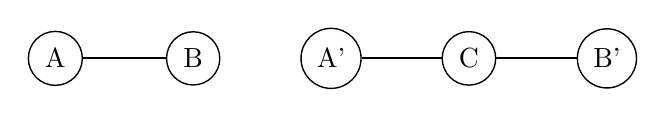
\begin{tikzpicture}[scale=1.75]
\GraphInit[vstyle=Normal]
\Vertex{A} \EA(A){B} \EA(B){A'} \EA(A'){C} \EA(C){B'}
\Edge(A)(B) \Edges(A',C,B')
\end{tikzpicture}
\end{center}

An \emph{edge contraction} is an operation which removes an edge of a graph while merging the vertices it used to connect. In other words, it is the result of replacing the edge joining vertices $A$ and $B$, as well as the vertices themselves, with a new vertex $C$, such that $C$ is joined to all the vertices $A$ and $B$ were joined to.

We say a graph $H$ is a \emph{minor} of another graph $G$ if we can obtain $H$ from $G$ after contracting some edges, deleting some edges, and afterwards deleting the vertices not joined to any other vertices. In the following diagram, the first graph is a minor of a second. The third graph illustrates this: the gray edge is deleted, the dashed edges are contracted, and the vertices that aren't joined to any other vertices are removed.

\begin{center}
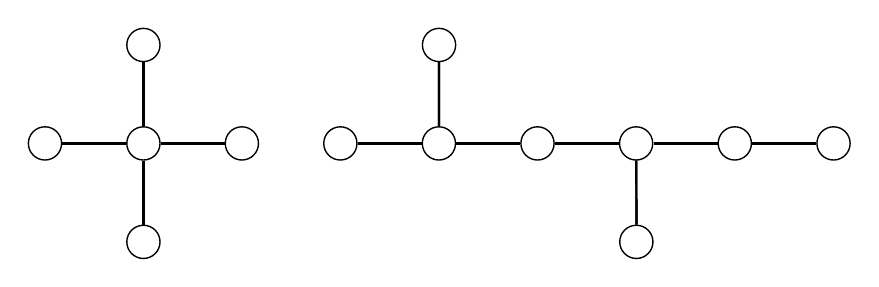
\begin{tikzpicture}[scale=1.25]
\GraphInit[vstyle=Hasse]
\Vertex{A} \NO(A){B} \WE(A){C} \EA(A){D} \SO(A){E}
\EA(D){C'} \EA(C'){A'} \NO(A'){B'} \EA(A'){F'} \EA(F'){D'}
\SO(D'){E'} \EA(D'){G'} \EA(G'){H'}
\Edges(A,B,A,C,A,D,A,E) \Edges(C',A',B',A',F',D',E',D',G',H')
\end{tikzpicture}
\end{center}
\begin{center}
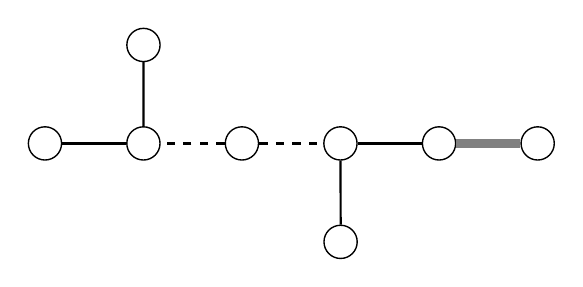
\begin{tikzpicture}[scale=1.25]
\GraphInit[vstyle=Hasse]
\Vertex{C'} \EA(C'){A'} \NO(A'){B'} \EA(A'){F'} \EA(F'){D'}
\SO(D'){E'} \EA(D'){G'} \EA(G'){H'}
\Edges(C',A',B') \Edges(E',D',G')
\Edge[style=dashed](F')(A')
\Edge[style=dashed](F')(D')
\draw (G') node {} -- (H') [color=gray, line width=3pt] node {};
\end{tikzpicture}
\end{center}

Definitions aside, we can now present Kuratowski's and Wagner's theorems:

\begin{theorem}[Kuratowski's theorem]
A graph is planar if and only if it does not contain a subdivision of $K_5$ or $K_{3,3}$ as a subgraph.
\end{theorem}

\begin{theorem}[Wagner's theorem]
A graph is planar if and only if neither $K_5$ nor $K_{3,3}$ is its minor.
\end{theorem}

Kuratowski's theorem was proved in 1930 by Kazimierz Kuratowski, and the proof is somewhat above the level of this article, and is omitted: a proof is listed as further reading. \cite{makarychev} It was independently proved by Orrin Frink and Paul Smith, also in 1930, but their proof was never published. 

Wagner's theorem was published in 1937 by Klaus Wagner, seven years after Kuratowski's publication. The proof is once again above the scope of this article, and a proof is listed as further reading. \cite{chudnovsky}

These theorems are both of interest because they are quite related to one another. Both are characterizations of planar graphs, both involving $K_5$ and $K_{3,3}$. To this extent, we can say that $K_5$ and $K_{3,3}$ are the roots of all non-planarity: we merely need to prove the non-planarity of both, then we can use either theorem to prove the non-planarity of any other non-planar graph.

\begin{center}
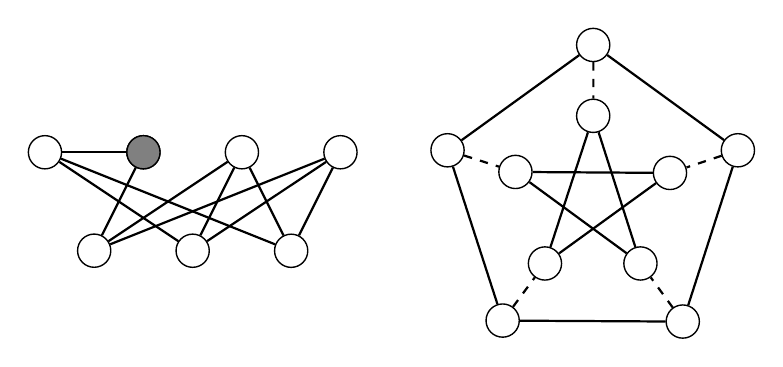
\begin{tikzpicture}[scale=1.25]
\GraphInit[vstyle=Hasse]
\Vertex{1} \EA(1){1'} \EA(1'){2} \EA(2){3}
\Vertex[x=.5,y=-1]{G} \EA(G){W} \EA(W){E}
\Edges(G,2,W,1,E,2) \Edges(1,1',G,3) \Edge(3)(W) \Edge(3)(E)
\AddVertexColor{gray}{1'}

\Vertex[x=5.57,y=1.09]{A1} \Vertex[x=7.04,y=0.02]{A2} \Vertex[x=6.48,y=-1.72]{A3} \Vertex[x=4.65,y=-1.71]{A4} \Vertex[x=4.09,y=0.02]{A5}
\Vertex[x=5.57,y=0.37]{B1} \Vertex[x=6.35,y=-0.21]{B2} \Vertex[x=6.05,y=-1.13]{B3} \Vertex[x=5.08,y=-1.13]{B4} \Vertex[x=4.78,y=-0.2]{B5} 
\Edges(A1,A2,A3,A4,A5,A1) \Edges(B1,B3,B5,B2,B4,B1)
\Edge[style=dashed](A1)(B1) \Edge[style=dashed](A2)(B2) \Edge[style=dashed](A3)(B3) \Edge[style=dashed](A4)(B4) \Edge[style=dashed](A5)(B5) 
\end{tikzpicture}
\end{center}

Observe the graph on the left in the above diagram. It has neither $K_5$ nor $K_{3,3}$ as its subgraph, however, we note that it is a subdivision of $K_{3,3}$. We note that the gray vertex subdivides an edge, and that removing this gray vertex gives us $K_{3,3}$. Therefore, the graph on the left is not planar.

On the other hand, observe the graph on the right. It is a graph known as the \emph{Petersen graph}, one of the more well-known graphs in graph theory. We can see that by contracting the dashed edges, we produce $K_5$, thus $K_5$ is a minor of the Petersen graph, meaning it is non-planar. The interested reader can also try to prove that $K_{3,3}$ is a minor of the Petersen graph for an alternate proof of non-planarity. 

\section{F\'{a}ry's theorem}

Suppose we have a planar drawing of a graph. Intuitively, we can find a planar drawing that uses only straight lines by ``stretching out'' the vertices, so that the curves can be replaced with straight lines without creating crossings. One might expect that every planar graph has a planar drawing using only straight lines.

This is, in fact, F\'{a}ry's theorem. The proof we present of F\'{a}ry's theorem does not in fact use the above intuition in its proof, but it confirms it. The proof itself uses several heuristics we have already discussed before, and we will go through these.

F\'{a}ry's theorem was named after Istv\'{a}n F\'{a}ry, who discovered it in 1948. It was proved independently by Klaus Wagner in 1936 and S. K. Stein in 1951. The proof we present is a common one found in graph theory textbooks.

Define a \emph{maximally planar} graph as a planar graph where we cannot add any edges while preserving planarity. A maximally planar graph is also called a \emph{triangulation of the plane}, the reason being the following problem, which the reader can easily prove:

\begin{problem}
Prove that every face in a maximally planar graph is enclosed by exactly three edges.
\end{problem}

\begin{proof}
Suppose for the sake of contradiction that there exists a face that is enclosed by more than three edges. Then we can draw another edge to split that face in two, while preserving planarity, contradicting the fact that the graph is maximally planar.
\end{proof}

We use the intuition of symmetry, that symmetric graphs are easier to work with that non-symmetric ones. In general, symmetric objects are easier to manipulate than asymmetric objects. Symmetric objects also have more properties than asymmetric ones. In this case, the symmetry is through maximally planar graphs. Maximally planar graphs are easier to work with than planar graphs, and there is a transformation that can change a planar graph to a maximally planar one, and vice-versa: just add or remove some edges.

Thus, we need only prove F\'{a}ry's theorem for the case of maximally planar graphs. Given, in general, a planar graph, we can add edges to make the graph maximally planar. Then we prove that this maximally planar graph has a straight-line drawing, and then remove the edges that we added in to give the original graph. Note that removing an edge does not change the fact that we have a straight-line drawing, so this is legal.

The idea behind F\'{a}ry's theorem is an induction on the number of vertices of the graph. How do we get from a maximally planar graph with $V + 1$ vertices to a maximally planar graph with $V$ vertices? We drop a vertex. If we can find a straight-line drawing of the graph with $V$ vertices, we only need to find a place for the new vertex such that a maximally planar graph with $V + 1$ vertices has a straight-line drawing as well.

We have the idea and the intuition of the proof nailed down. Now we only need formalize it. We first prove the following useful (and interesting) theorem, that allows us to find a place for the new vertex such that there is a straight-line drawing of it. This is an interesting result, and the reader is once again encouraged to try and prove this before reading our presented proof:

\begin{problem}[Art gallery theorem]
Given a polygon with $n$ vertices, prove that we can pick $\floor{\frac{n}{3}}$ points on it such that we can draw a line segment from any polygon vertex to one of these $\floor{\frac{n}{3}}$ points without the line segment leaving the polygon.
\end{problem}

\begin{center}
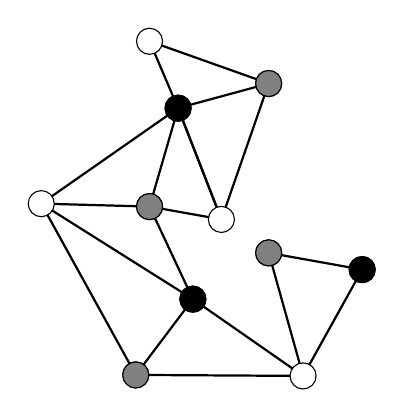
\begin{tikzpicture}[scale=1.25]
\GraphInit[vstyle=Hasse]
\tikzset{VertexStyle/.style = {shape = circle, minimum size = 6 pt, draw}}
\Vertex[x=0.14,y=3.39]{1} \Vertex[x=1.35,y=2.96]{2} \Vertex[x=0.43,y=2.71]{3} \Vertex[x=-0.96,y=1.74]{4} \Vertex[x=0.14,y=1.71]{5} \Vertex[x=0.87,y=1.58]{6} \Vertex[x=1.35,y=1.24]{7} \Vertex[x=2.3,y=1.07]{8} \Vertex[x=0.58,y=0.77]{9} \Vertex[x=0,y=0]{10} \Vertex[x=1.7,y=-0.01]{11} 
\Edges(1,2,3,1) \Edges(2,6,3,5,6,3,4,5,9,4,10,9,11) \Edges(10,11,7,8,11)
\AddVertexColor{gray}{2,5,7,10}
\AddVertexColor{black}{3,8,9}
\end{tikzpicture}
\end{center}

\begin{proof}
Triangulate the polygon, and color the vertices of the resulting triangulation with three colors. Pick the color with the least number of vertices of that color: there are at most $\floor{\frac{n}{3}}$ of these vertices by the pigeonhole principle. These points are such a set of $\floor{\frac{n}{3}}$ points. For any vertex, we just pick a triangle containing that vertex, and then pick the vertex in that triangle of the color we chose -- the resulting line segment does not escape the polygon, as it is one of the triangle's sides.
\end{proof}

The theorem's colorful name comes from its original combinatorial phrasing: the polygon is an art gallery, and the points chosen are guards. The problem was to pick places for the guards to stand such that every point in the art gallery has at least one guard in its line of sight.

We are nearly done. We just need to think about how to do the induction step. How do we get from a straight-line drawing with $V$ vertices to a straight-line drawing with $V + 1$ vertices? First, we have to pick a place for the vertex. Second, we draw in the edges connecting that vertex to the existing vertices. The second step is handled by the art gallery theorem: if we have a polygon with less than or equal to five sides, we can pick one point on it so that point can be connected to all of the polygon's vertices with straight lines.

We need a polygon with less than or equal to five sides, for the vertex to be placed in. If we have a graph with $V + 1$ vertices, we need to look for a vertex connected to not more than five other vertices, remove that vertex, use the induction to find a straight-line drawing for $V$ vertices, add that vertex in, and then use the art gallery theorem to find a straight-line drawing. But there is a catch: this vertex can't be connected to any of the outer faces, because otherwise we can't use the art gallery theorem.

To deal with this catch, we pick three vertices before hand that would form the outer face of the straight-line drawing. This makes our argument even stronger: instead of finding a straight-line drawing of $V$, our induction wants to show that there is a straight-line drawing of $V$ with three selected vertices that would be the outer face of that drawing.

Once we find a point connected to less than or equal to five vertices, and not connected to any of the three vertices that would form the outer face, we can do the induction step on that vertex. The trouble is, is there always such a vertex? For a planar graph, yes: we use a result from the previous sections to prove so. The reader is encouraged to try to prove the following:

\begin{problem}
Any planar graph has a vertex connected at most five other vertices, not connected to three vertices chosen beforehand.
\end{problem}

\begin{proof}
Let the graph have $V$ vertices. Suppose otherwise: that all $V-3$ vertices are connected to at least six other vertices. This does not count the three vertices chosen, which have to be connected to at least one other vertex, as the graph is connected.

We then count the total number of edges: $E > \frac{6(V-3)}{2} + 3 = 3V - 6$. The first term comes from multiplying the number of vertices by six, then dividing by two as we double counted. The second term comes from the three vertices we picked, which have to be connected to at least one other vertex each. Note that the inequality is strict: if equality held, we wouldn't have a planar graph.

Now this inequality $E > 3V - 6$ contradicts the earlier proven fact, that for planar graphs, $E \leq 3V - 6$. Thus there exists a vertex connected to at most five other vertices, not connected to the three vertices we picked.
\end{proof}

At this point, our proof of F\'{a}ry's theorem is pretty much done. We just need to write it up nicely, which the reader is encouraged to try out:

\begin{problem}[F\'{a}ry's theorem]
Any planar graph has a straight line drawing.
\end{problem}

\begin{proof}
We prove a stronger statement: that every maximally planar graph has a straight-line drawing that has three vertices picked beforehand as the outer face. We do induction on the number of vertices. The base case is when the graph has three vertices, the proof is trivial.

Suppose a graph $G$ has $V$ vertices, and assume it is maximally planar. If it is not maximally planar, we add edges to make it maximally planar, and then we can delete them afterwards. Choose three vertices that would form the outer face of the straight-line drawing.

\begin{center}
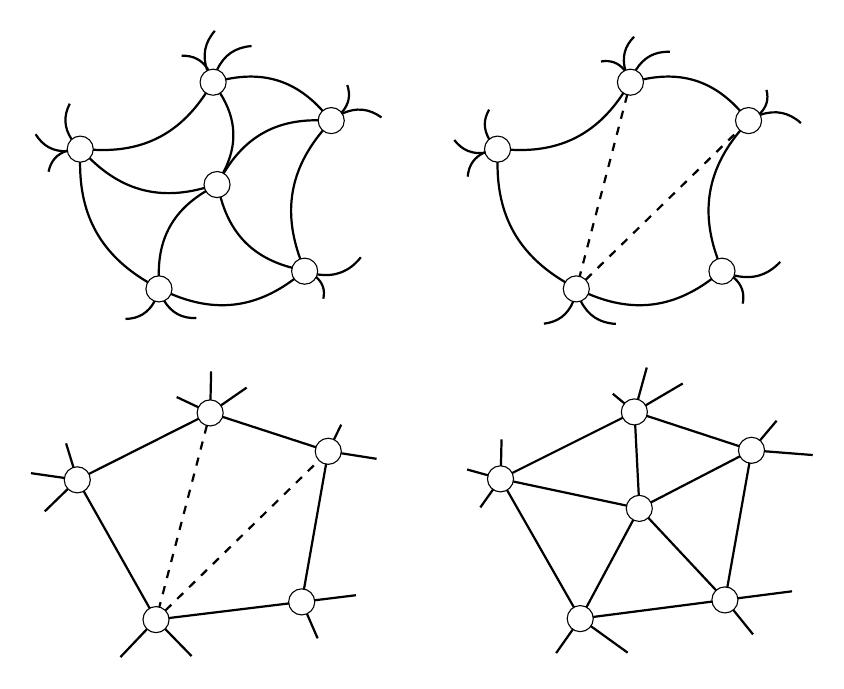
\begin{tikzpicture}[scale=1.25]
\GraphInit[vstyle=Hasse]
\tikzset{VertexStyle/.style = {shape = circle, minimum size = 6 pt, draw}}
\Vertex[x=1.14,y=5.86]{A1} \Vertex[x=2.34,y=5.47]{A2} \Vertex[x=2.07,y=3.94]{A3} \Vertex[x=0.59,y=3.76]{A4} \Vertex[x=-0.21,y=5.18]{A5} \Vertex[x=1.18,y=4.82]{A6}
\Vertex[x=5.38,y=5.86]{B1} \Vertex[x=6.58,y=5.47]{B2} \Vertex[x=6.31,y=3.94]{B3} \Vertex[x=4.83,y=3.76]{B4} \Vertex[x=4.03,y=5.18]{B5}
\Vertex[x=1.11,y=2.5]{C1} \Vertex[x=2.31,y=2.11]{C2} \Vertex[x=2.04,y=0.58]{C3} \Vertex[x=0.56,y=0.4]{C4} \Vertex[x=-0.24,y=1.82]{C5}
\Vertex[x=5.42,y=2.51]{D1} \Vertex[x=6.61,y=2.12]{D2} \Vertex[x=6.34,y=0.6]{D3} \Vertex[x=4.87,y=0.41]{D4} \Vertex[x=4.06,y=1.83]{D5} \Vertex[x=5.47,y=1.53]{D6}
\Edge[style={bend left}](A1)(A2) \Edge[style={bend right}](A2)(A3) \Edge[style={bend left}](A3)(A4) \Edge[style={bend left}](A4)(A5) \Edge[style={bend right}](A5)(A1)
\Edge[style={bend left}](A1)(A6) \Edge[style={bend right}](A2)(A6) \Edge[style={bend left}](A3)(A6) \Edge[style={bend left}](A4)(A6) \Edge[style={bend right}](A5)(A6)
\Edge[style={bend left}](B1)(B2) \Edge[style={bend right}](B2)(B3) \Edge[style={bend left}](B3)(B4) \Edge[style={bend left}](B4)(B5) \Edge[style={bend right}](B5)(B1)
\Edges[style=dashed](B1,B4,B2)
\Edges(C1,C2,C3,C4,C5,C1) \Edges[style=dashed](C1,C4,C2)
\Edges(D1,D2,D3,D4,D5,D1) \Edge(D1)(D6) \Edge(D2)(D6) \Edge(D3)(D6) \Edge(D4)(D6) \Edge(D5)(D6) 

\Vertex[empty,x=1.17,y=6.4]{W7} \Vertex[empty,x=1.55,y=6.23]{W8} \Vertex[empty,x=2.5,y=5.85]{W9} \Vertex[empty,x=2.87,y=5.49]{W10} \Vertex[empty,x=2.66,y=4.1]{W11} \Vertex[empty,x=2.26,y=3.64]{W12} \Vertex[empty,x=0.99,y=3.46]{W13} \Vertex[empty,x=0.23,y=3.45]{W14} \Vertex[empty,x=-0.54,y=4.93]{W15} \Vertex[empty,x=-0.68,y=5.35]{W16} \Vertex[empty,x=-0.31,y=5.66]{W17} \Vertex[empty,x=0.8,y=6.13]{W18} 
\Edges[style={bend left}](W18,A1,W7) \Edge[style={bend left}](A1)(W8) \Edges[style={bend left}](W9,A2,W10) \Edges[style={bend left}](W11,A3,W12) \Edges[style={bend left}](W13,A4,W14) \Edges[style={bend left}](W15,A5,W16) \Edge[style={bend left}](A5)(W17) 

\Vertex[empty,x=5.43,y=6.34]{X7} \Vertex[empty,x=5.8,y=6.17]{X8} \Vertex[empty,x=6.76,y=5.8]{X9} \Vertex[empty,x=7.13,y=5.43]{X10} \Vertex[empty,x=6.92,y=4.05]{X11} \Vertex[empty,x=6.52,y=3.59]{X12} \Vertex[empty,x=5.25,y=3.4]{X13} \Vertex[empty,x=4.48,y=3.4]{X14} \Vertex[empty,x=3.72,y=4.88]{X15} \Vertex[empty,x=3.57,y=5.29]{X16} \Vertex[empty,x=3.95,y=5.6]{X17} \Vertex[empty,x=5.06,y=6.07]{X18}
\Edges[style={bend left}](X18,B1,X7) \Edge[style={bend left}](B1)(X8) \Edges[style={bend left}](X9,B2,X10) \Edges[style={bend left}](X11,B3,X12) \Edges[style={bend left}](X13,B4,X14) \Edges[style={bend left}](X15,B5,X16) \Edge[style={bend left}](B5)(X17)

\Vertex[empty,x=1.12,y=2.94]{Y7} \Vertex[empty,x=1.5,y=2.77]{Y8} \Vertex[empty,x=2.45,y=2.4]{Y9} \Vertex[empty,x=2.82,y=2.03]{Y10} \Vertex[empty,x=2.61,y=0.65]{Y11} \Vertex[empty,x=2.21,y=0.19]{Y12} \Vertex[empty,x=0.94,y=0.01]{Y13} \Vertex[empty,x=0.18,y=0]{Y14} \Vertex[empty,x=-0.59,y=1.48]{Y15} \Vertex[empty,x=-0.73,y=1.89]{Y16} \Vertex[empty,x=-0.36,y=2.21]{Y17} \Vertex[empty,x=0.75,y=2.67]{Y18} 
\Edges(Y18,C1,Y7) \Edge(C1)(Y8) \Edges(Y9,C2,Y10) \Edges(Y11,C3,Y12) \Edges(Y13,C4,Y14) \Edges(Y15,C5,Y16) \Edge(C5)(Y17)

\Vertex[empty,x=5.55,y=2.98]{Z7} \Vertex[empty,x=5.93,y=2.81]{Z8} \Vertex[empty,x=6.88,y=2.44]{Z9} \Vertex[empty,x=7.25,y=2.07]{Z10} \Vertex[empty,x=7.04,y=0.69]{Z11} \Vertex[empty,x=6.64,y=0.23]{Z12} \Vertex[empty,x=5.37,y=0.05]{Z13} \Vertex[empty,x=4.61,y=0.04]{Z14} \Vertex[empty,x=3.84,y=1.52]{Z15} \Vertex[empty,x=5.18,y=2.71]{Z18} \Vertex[empty,x=3.7,y=1.93]{Z16} \Vertex[empty,x=4.07,y=2.25]{Z17}
\Edges(Z18,D1,Z7) \Edge(D1)(Z8) \Edges(Z9,D2,Z10) \Edges(Z11,D3,Z12) \Edges(Z13,D4,Z14) \Edges(Z15,D5,Z16) \Edge(D5)(Z17)
\end{tikzpicture}
\end{center}

For the induction step, pick any vertex $v$ such that at most five vertices are connected to $v$ by an edge, and $v$ is not connected to the three vertices we picked beforehand, which is possible by a previous result. We remove $v$ from the graph $G$ to create another graph, $G'$.

We triangulate the face created by removing $v$. This creates a maximally planar graph with one less vertex than $G$, which can be drawn with straight lines by induction hypothesis. We remove the edges created by triangulation, then put back $v$ in this face, choosing the $\floor{\frac{5}{3}} = 1$ point given by the art gallery theorem. Then connect $v$ to the vertices of this face, giving back a straight-line drawing of $G$.
\end{proof}

\section{The crossing number inequality}

Intuitively, if we have a graph, fix the number of vertices, and increase the number of edges, the graph should become ``increasingly non-planar'': the more edges we add, the more crossings the graph should have. Our intuition says that planarity is dependent on the number of edges and the number of vertices.

Such an intuition was formalized by the crossing number inequality, discovered by Ajtai, Chv\'{a}tal, Newborn and Szemer\'{e}di, and independently by Leighton. We present a probabilistic argument here, beginning with a weak bound of $\crs{G}$, to a stronger bound with the requirement of $E \geq 4V$. Much discussion is borrowed from \cite{tao}.

We begin with a lemma, a corollary of the fact that, for planar graphs, $E \leq 3V - 6$:

\begin{problem}
For any graph $G$, show that $\crs{G} \geq E - 3V$.
\end{problem}

\begin{proof}
Note that every crossing is made by two edges: if a crossing is only made by one edge in an $\alpha$ shape, then we can just flip the edge to reduce the number of crossings. For each crossing, we remove one of the edges over that crossing. This makes a new graph $G'$ with at most $E' = E - \crs{G}$ edges, and has the same number $V$ of vertices. But then the operation makes $G'$ planar: all of its crossings are gone! Since $G'$ is planar, it satisfies the inequality $E' \leq 3V' - 6$, thus for any graph $G$, we have $E - \crs{G} \leq 3V - 6$, or simply $\crs{G} \geq E - 3V$.
\end{proof}

Now, what is the motivation for this? We are given a graph $G$, and we wish to find an inequality involving $\crs{G}, E,$ and $V$. We look back to our known results, and we remember that, for planar graphs, $E \leq 3V - 6$. But most graphs aren't planar.

We apply the technique that Terence Tao described as \emph{amplification}: given an object, we use a transformation to make it into a new object, apply an estimate to the new object, and see what it says about the original. In this case, like many others, we begin with an ``asymmetric'' object, a graph $G$ which is non-planar, and transform it into something ``symmetric'', a planar graph $G'$. We then apply what we know about the symmetric object to deduce a fact about the asymmetric object.

Once again, the heuristic of \emph{exploiting symmetry} is used. Another heuristic done in this solution is \emph{exploiting freedom}: given the freedom to delete edges, we do so. And again, the heuristic of decomposition and recomposition appears, when we decomposed a non-planar graph into a planar one.

We once again apply amplification, and again exploit a freedom, this time to delete vertices. However, there is no easy symmetric way to do so -- if we delete vertices connected to crossings, we might delete edges not in crossings, which is inefficient. Without any easy way to use symmetry, we proceed with the \emph{probabilistic method}.

\begin{theorem}[Crossing number inequality]
For any graph $G$ satisfying $E \geq 4V$, we have $\crs{G} \geq \dfrac{E^3}{64V^2}$.
\end{theorem}

\begin{proof}
Consider the fact that $\crs{G} \geq E - 3V$. We randomly pick vertices to remove, with the probability of a vertex remaining being $0 < p < 1$, to create a new graph $G'$ with $E'$ edges and $V'$ vertices. By the inequality, we have $\crs{G'} \geq E' - 3V'$. We use linearity of expectation to get $\EE(\crs{G'}) \geq \EE(E') - 3\EE(V')$.

These are easy to compute: $\EE(V')$ is simply $pV$, since each vertex has probability $p$ to remain in $G'$. For the edges, we have $\EE(E') = p^2E$, as an edge remains if both endpoints remain in $G'$. Each endpoint has probability $p$ to remain, so the probability that an edge remains is $p^2$.

Finally, we compute $\EE(\crs{G'})$. Note that a crossing involves two edges, and thus, four vertices. Thus the probability a crossing remains in $G'$ is $p^4$, the probability that its four vertices all remain. We get $\EE(\crs{G'}) \leq p^4\crs{G}$, an inequality because the current drawing may not be the optimal one.

After substituting to the inequality and dividing by $p^4$, we get $\crs{G} \geq p^{-2}E - 3p^{-3}V$. Finally, since $E \geq 4V,$ it is possible to choose $p$ such that $4p^{-3}V = p^{-2}E$. This gives $\crs{G} \geq \frac{E^3}{64V^2}$, which was what we wanted.
\end{proof}

The crux idea in the proof was the probabilistic method, a tool that has found helpful use in combinatorics, in Ramsey theory and incidence geometry, for example. The probabilistic method is a helpful tool when it comes to olympiad-flavored problems, and an article about it is listed as further reading. \cite{chen}

One aspect of the proof which may require motivation is the choice of $p$. We have the inequality $\crs{G} \geq p^{-2}E - 3p^{-3}V$, and we wish to make this inequality sharp. Generally, inequalities are sharp when the terms are roughly in balance, because we get closer to the equality case. We want to make the two terms here, $p^{-2}E$ and $3p^{-3}V$ in balance -- we want to make the latter term only slightly smaller than the former.

This is where the restriction, $E \geq 4V$, comes in. This restriction was not arbitrary: we chose the restriction so that $4p^{-3}V = p^{-2}E$ is the conclusion, and thus the two terms we wanted to balance are fairly close to each other.

Sz\'{e}kely wrote a paper illustrating several proofs that the crossing number inequality gives to hard combinatorial incidence geometry theorems. \cite{szekely} We present the Szemer\'{e}di-Trotter theorem below, as its proof is one of the most elementary of Sz\'{e}kely's. It is a direct application of the inequality.

\begin{theorem}[Szemer\'{e}di-Trotter theorem]
Given $P$ points and $L$ lines, the maximum number of incidences between them is $O(L^{2/3}P^{2/3} + P + L)$.
\end{theorem}

\begin{proof}
Let $I(P, L) = |\{(p, l) \in P \times L : p \in l\}|$ be the number of incidences, or the number of distinct pairs of points and lines $(p, l)$ such that point $p$ lies on line $l$.

We make the observation that the points and lines naturally determine a graph. Assume for the moment that each line is incident to at least two points. We observe that for a single line $l$ that has $n$ points on it, these $n$ points have $n-1$ segments in between them. Since the sum of all the $n$ for all lines is $I(P, L)$ by definition, then the sum of the number of line segments between the points is similar to $I(P, L)$.

Thus these points and lines produce a graph with $P$ vertices and about $I(P, L)$ edges. We count the number of crossings. Since two lines intersect in at most one point, the number of crossings has to be approximately $L^2$. Applying the crossing number inequality gives us $L^2 = O(I(P, L)^3 / P^2)$, if $I(P, L)$ is larger than $P$.

This leads to $I(P, L) = O(L^{2/3}P^{2/3} + P)$. Then we remove our assumption that each line is incident to at least two points, by observing that lines incident to one point contribute at most $L$ incidences. Thus, $I(P, L) = O(L^{2/3}P^{2/3} + P + L)$.
\end{proof}

\section{Conclusions}

We conclude with a few remarks about crossing numbers. Note that in the third dimension, we can always draw a graph with zero crossings, but what about on other surfaces, like toruses? We leave to the interested reader to discover that graphs which are not planar in the Euclidean plane are planar on other surfaces.

Plenty of other developments have been found on crossing numbers that is not discussed here. Bounds on crossing numbers have been obtained on complete bipartite graphs and complete graphs. Improvements have been found for the crossing number inequality: changing the condition $E > 7V$ gives the improvement $\crs{G} \geq \frac{E^3}{29V^2}$, which is the best known constant to date.

There are also several open problems on planar graphs that the reader can look into. (And for the more daring and ambitious readers, open problems to attempt!) Graph theory, unlike other fields of mathematics, has a relatively lower amount of prerequisite knowledge required. On the other hand, it also requires far more creativity.

The writer would like to acknowledge the contributions of Sean Ty and Ivan Chan for looking over a draft of the article. If you see an error, have a correction or an addition, or have a question, you can reach me at \mailto{cj@cjquines.com}.

\section{Problems}

\begin{problem}
We know that $\crs{K_4} = 0$ and $\crs{K_5} = 1$. What about $\crs{K_6}$? Does a similar argument work? Can you find bounds on $\crs{K_7}$?
\end{problem}

\begin{problem}
What about $\crs{K_{3,4}}, \crs{K_{3,5}}$ and $\crs{K_{4,4}}$?
\end{problem}

\begin{problem}
Three graphs are presented below. Which ones are planar and which ones are not? Prove your claims.
\end{problem}

\begin{center}
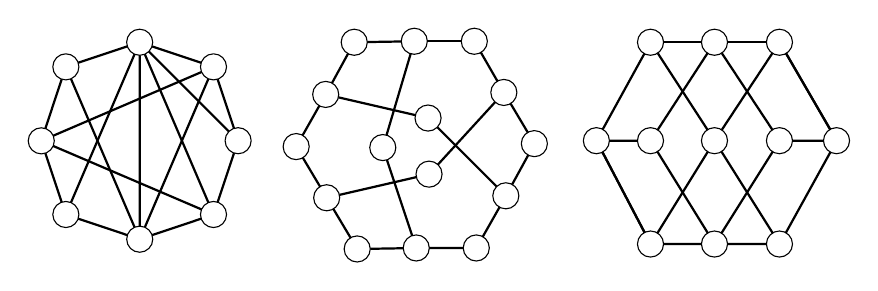
\begin{tikzpicture}[scale=1.25]
\GraphInit[vstyle=Hasse]
\tikzset{VertexStyle/.style = {shape = circle, minimum size = 4 pt, draw}}

\Vertex{1} \SOEA(1){3} \SOWE(3){5} \NOWE(5){7}
\Vertex[x=.75, y=-.25]{2} \Vertex[x=-.75, y=-.25]{8}
\Vertex[x=.75, y=-1.75]{4} \Vertex[x=-.75, y=-1.75]{6}
\Edges(1,2,3,4,5,6,7,8,5,2,7,4,1,5) \Edges(8,1,3) \Edge(1)(6)

\Vertex[x=2.18,y=0]{A1} \Vertex[x=2.79,y=0.01]{A2} \Vertex[x=3.4,y=0.01]{A3} \Vertex[x=3.7,y=-0.51]{A4} \Vertex[x=4.01,y=-1.03]{A5}
\Vertex[x=3.72,y=-1.56]{A6} \Vertex[x=3.42,y=-2.09]{A7} \Vertex[x=2.81,y=-2.09]{A8} \Vertex[x=2.21,y=-2.1]{A9} \Vertex[x=1.9,y=-1.58]{A10}
\Vertex[x=1.59,y=-1.06]{A11} \Vertex[x=1.89,y=-0.53]{A12} \Vertex[x=2.93,y=-0.77]{A13} \Vertex[x=2.47,y=-1.07]{A14} \Vertex[x=2.94,y=-1.34]{A15}
\Edges(A1,A2,A3,A4,A5,A6,A7,A8,A9,A10,A11,A12,A1) \Edges(A12,A13,A6) \Edges(A2,A14,A8) \Edges(A4,A15,A10)

\Vertex[x=5.19,y=0]{B1} \Vertex[x=5.84,y=0]{B2} \Vertex[x=6.5,y=0]{B3} \Vertex[x=4.64,y=-1]{B4} \Vertex[x=5.19,y=-1]{B5}
\Vertex[x=5.84,y=-1]{B6} \Vertex[x=6.5,y=-1]{B7} \Vertex[x=7.08,y=-1]{B8} \Vertex[x=5.19,y=-2.05]{B9} \Vertex[x=5.84,y=-2.05]{B10} \Vertex[x=6.5,y=-2.05]{B11}
\Edges(B1,B2,B3,B8,B11,B10,B9,B4,B1) \Edges(B1,B6,B9,B4,B5,B2,B7,B10,B5) \Edges(B7,B8,B3,B6,B11)
\end{tikzpicture}
\end{center}

\begin{problem}
Are $K_{3,3}$ and $K_5$ planar on a torus? What about on a Klein bottle?
\end{problem}

\begin{problem}
More generally, are all graphs $G$ such that $\crs{G} \leq 1$ planar on a torus? What about on a Klein bottle? Can you come up with an example of a graph with $\crs{G} \geq 2$ that is planar on a torus?
\end{problem}

\begin{problem}
Even more generally, are all graphs that are planar on a torus also planar on a Klein bottle? Why or why not?
\end{problem}

\begin{thebibliography}{99}

\bibitem{chen} Chen's handout on the probabilistic method at \url{http://www.mit.edu/~evanchen/handouts/ProbabilisticMethod/ProbabilisticMethod.pdf}.

\bibitem{chudnovsky} Chudnovsky et al.'s paper on bipartite minors, which includes a proof of Wagner's theorem at \url{http://mfleck.cs.illinois.edu/building-blocks/version-1.0/planargraphs.pdf}.

\bibitem{fleck} A portion of Fleck's book on planar graphs, which includes a discussion of the Euler characteristic and Platonic solids at \url{http://mfleck.cs.illinois.edu/building-blocks/version-1.0/planargraphs.pdf}.

\bibitem{makarychev} Makarychev's short proof of Kuratowski's theorem at \url{http://ttic.uchicago.edu/~yury/papers/kuratowski.pdf}.

\bibitem{szekely} Sz\'{e}kely's paper on using crossing numbers to prove hard problems in incidence geometry, at \url{http://www.cs.tau.ac.il/~michas/szekely.pdf}.

\bibitem{tao} Tao's post on the crossing number inequality, at \url{http://terrytao.wordpress.com/2007/09/18/the-crossing-number-inequality}.

\bibitem{wikipedia} A Wikipedia article on the Euler characteristic, at \url{https://en.wikipedia.org/wiki/Euler_characteristic}

\end{thebibliography}

\end{document}
